\section{Konzept}
\label{sec:concept}

In den vorangegangenen Kapiteln wurde zusammengefasst, was die Dateiverwaltung der Schul-Cloud leisten muss und woran sie sich orientieren kann. Vom Partner des Bachelor-Projekts MINT-EC \footnote{Verein mathematisch-naturwissenschaftlicher Excellence-Center an Schulen e. V. (MINT-EC) - \url{https://www.mint-ec.de/}}  und dem Hasso-Plattner-Institut wurde eine Anforderungsspezifikation erstellt, an welcher sich das folgende Konzept der Dateiverwaltung orientiert (Abbildung 2). Neben der Verwaltung von eigenen Dateien, sollen auch  jene im Kurs- bzw. Fächer- so wie Klassenkontext verteilbar sein. Dies soll dazu dienen, digitale Inhalte besser in den Unterricht einzubetten und (Haus)-Aufgaben mithilfe von anschaulichem Material zu gestalten. Somit sollen diese Dateien über eine einheitliche Schnittstelle durch die Backend-API sowie über das Web-Frontend in mehreren Kontexten verfügbar sein. Außerdem soll es für eine Schule möglich sein, eine bereits bestehende Dateiablage einzubinden. 

\begin{figure}[H]
	\centering
	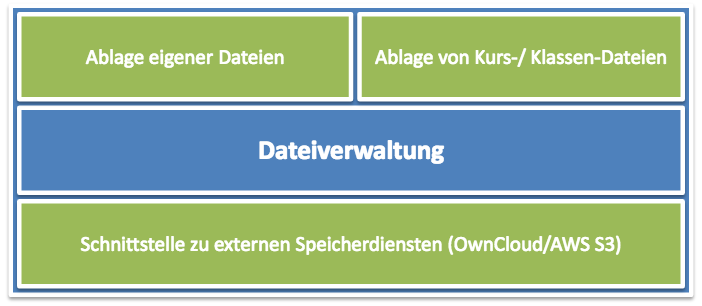
\includegraphics[width=0.8\linewidth]{images/AnforderungenDateiverwaltung}
	\caption[Caption for concept]{Grundanforderungen an die Dateiverwaltung der Schul-Cloud\footnotemark}
\end{figure}
\footnotetext{Martin Hense (Mint-EC - \url{https://www.mint-ec.de/})}


\subsection{Grundaufbau Dateiverwaltung}

\begin{figure}[H]
	\centering
	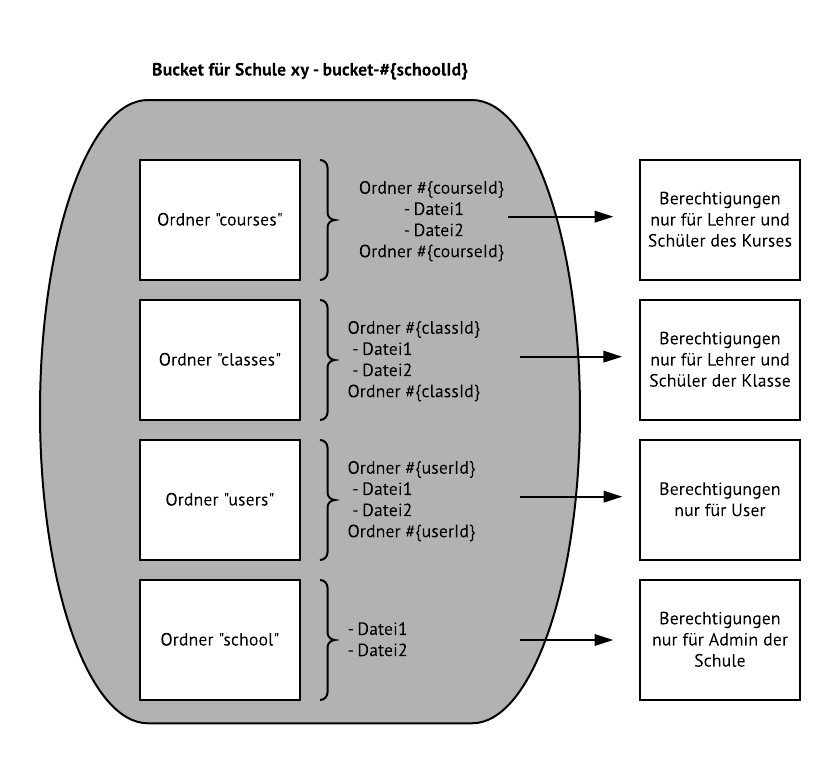
\includegraphics[width=0.8\linewidth]{images/AufbauDateiverwaltung}
	\caption[Caption for concept]{Grundaufbau eines Schul-Buckets}
\end{figure}

\subsection{Architektur verteilter Provider}

\begin{figure}[H]
	\centering
	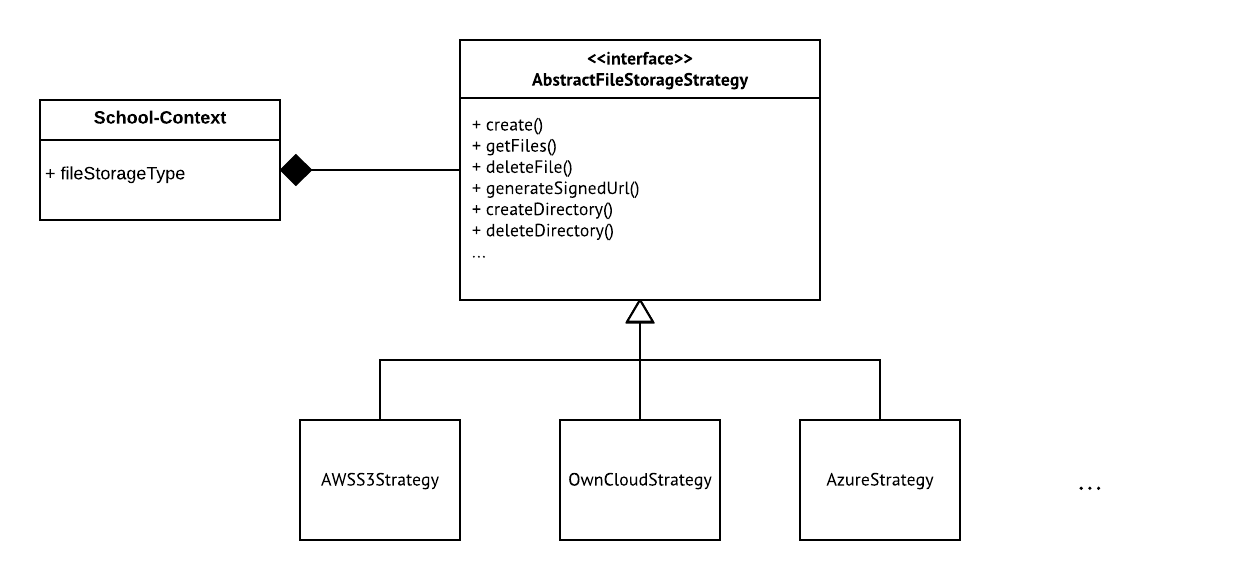
\includegraphics[width=1\linewidth]{images/strategypattern}
	\caption[Caption for concept]{Verteilung der Schul-Buckets mithilfe des Strategy-Patterns}
\end{figure}

\subsection{Interaktion verschiedener Schul-Cloud Komponenten}

\todo{Bilder Qualität verbessern!!}

\begin{figure}[H]
	\centering
	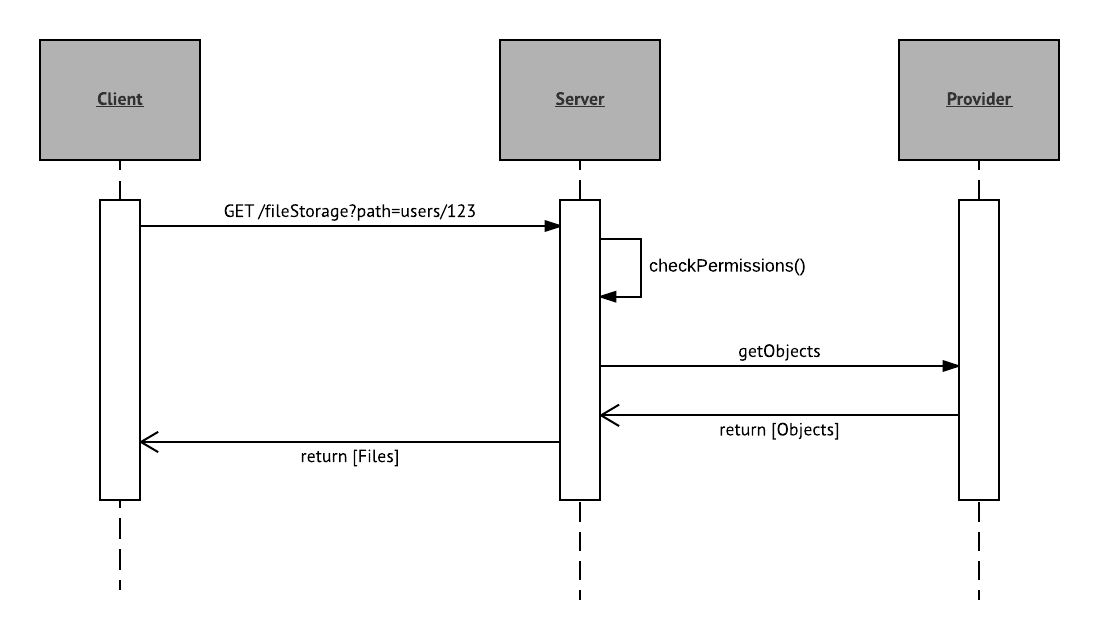
\includegraphics[width=1\linewidth]{images/fileumlsequence}
	\caption[Caption for concept]{Interaktion zwischen Client, Server und File Storage Provider}
\end{figure}


\subsection{Teilen von Dateien}

\begin{figure}[H]
	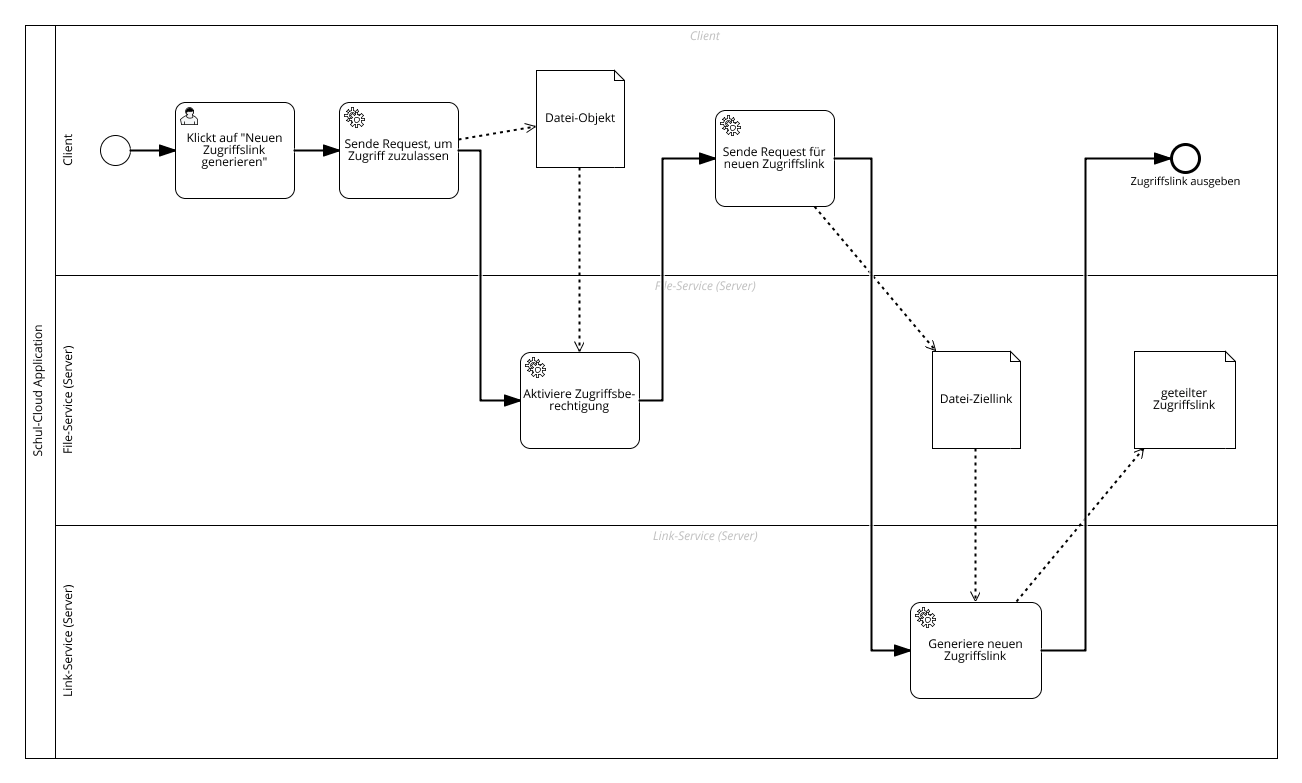
\includegraphics[width=1\linewidth]{images/filesharinggeneration}
	\caption[Caption for concept]{Generierung eines Zugriffslinks}
	\centering
\end{figure}

\begin{figure}[H]
	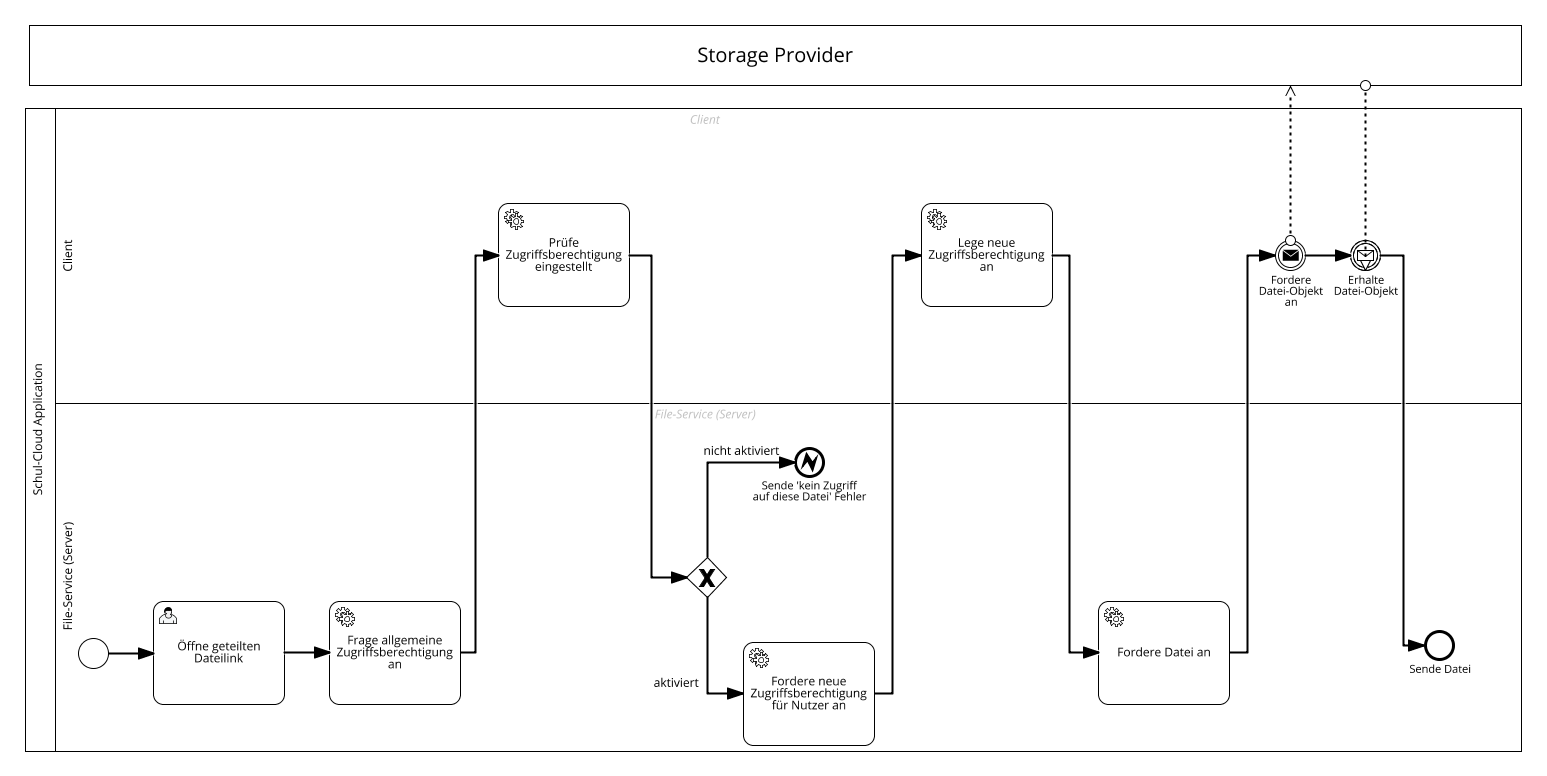
\includegraphics[width=1\linewidth]{images/filesharingusing}
	\caption[Caption for concept]{Zugriff auf eine geteilte Datei}
	\centering
\end{figure}


\clearpage
